\documentclass[marginline,answers]{BHCexam}
\usepackage{tkz-euclide}

\begin{document}
\biaoti{2023小升初考试数学试卷}
\fubiaoti{}
\maketitle

\begin{questions}
\tiankong
\question $a$是一个四位数,“四舍五入”取近似值为4.68,那么$a$的最大值是\stk{4.6849},最小值是\stk{4.6750}.

\question 等底等高的圆柱和圆锥的体积之差是40立方分米,圆柱的体积是\stk{60}立方分米.

\question 比45千克少$\dfrac{2}{5}$的是\stk{27}千克,\stk{200}千克比150千克多$\dfrac{1}{3}$.

\question 2075立方厘米=\stk{2.075}立方分米,1500平方米=\stk{0.15}公顷.

\question 甲乙两个齿轮齿数比为$3:5$,它们互相咬合,当甲齿轮转50圈时,乙齿轮转\stk{30}圈.

\question 在一个长8 cm,宽6 cm的长方形里画一个最大的半圆,这个半圆的周长是\stk{20.56}cm,面积是\stk{25.12} cm$^{2}$.

\begin{minipage}{0.7\textwidth}
	\question 某产品,不合格与合格的个数比是4:6,产品的合格率是\stk{60\%}.
	
	\question 如图是一个等腰直角三角形,它的面积是\stk{4.5}cm$^{2}$,把它以$AB$所在直线为轴旋转一周,形成的图形的体积是\stk{28.26}cm$^{2}$.
	
	\question 围棋组人数在30$\sim$ 40之间,男生与女生的人数比是5:7,围棋组有\stk{36}人.
\end{minipage}
\begin{minipage}{0.3\textwidth}
	\begin{center}
		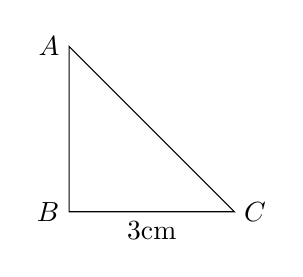
\begin{tikzpicture}[scale=0.7]
		\draw(0,0) node[left]{$B$}--(3,0)node[right]{$C$}--(0,3)node[left]{$A$}--cycle;
		\node[below] at(1.5,0) {3cm};
		\end{tikzpicture}
	\end{center}
\end{minipage}

\question 0.4:1.6的比值是\stk{0.25},如果前项加上0.8,要使比值不变,后项应加上\stk{3.2}.

\question \stk{扇形}统计图能反映各个部分在总体中所占的百分比.在一个这样的统计图中,某部分占总体的30\%,则该部分扇形的圆心角是\stk{108}$^\circ$.

\question 一个分数的分子增加20\%,而分母减少20\%,得到新的分数比原来的分数增加\stk{50\%}.

\question 一件100元的商品,降价5\%后又提价5\%,这时价格为\stk{99.75}.

\question 把一个棱长为8里米的正方形削成一个最大的圆柱体,这个圆柱体的表面积是\stk{301.44}平方厘米,削去的体积是\stk{110.08}立方厘米.

\question 如图,摆一个正六边形需要六根小棒,摆两个正六边形需要11根小棒,按这样摆下去,摆10个正六边形需要\stk{51}根小棒,摆$n$个正六边形需要\stk{5n+1}根小棒.

\begin{center}
	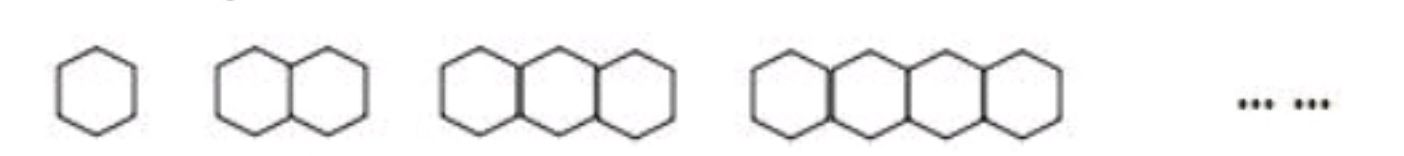
\includegraphics[scale=0.2]{tiankong}
\end{center}
\xuanze
\question 在浓度为10\%的1000克盐水中加入100克盐,溶解之后,盐与盐水的质量比为2:11.\xx{$\surd$}
\question 把一个圆柱体削成一个最大的圆锥体,圆锥体的体积是削去部分的一半.\xx{$\surd$}
\question 红糖重量比白糖多10\%,就是白糖重量比红糖少10\%.\xx{x}
\question 如果高铁行驶速度不变,则它所行驶的路程与所用时间成反比例.\xx{x}
\question 2024年第一季度有91天且这一年是闰年.\xx{$\surd$}

\xuanze

\question 乐器商店新进了9把小提琴,共花了3600元,售价合理的是\xx{B}

\onech{400把/元}{498元/把}{498把/元}{400元/把}

\begin{minipage}{0.8\textwidth}
	\question 一个圆和正方形的周长都是12.56厘米,比较它们的面积\xx{C}
	
	\onech{一样大}{正方形大}{圆大}{无法比较}
	
	\question 如图,下列比例式正确的是\xx{B}
	
	\onech{$a:b=c:h$}{$a:h=c:b$}{$b:c=h:a$}{$b:a=c:h$}
	
\end{minipage}
\begin{minipage}{0.2\textwidth}
	\begin{center}
		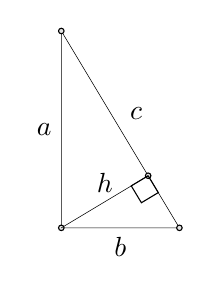
\begin{tikzpicture}
		\tkzDefPoints{0/0/A,1.5/0/B,0/2.5/C}
		\tkzDrawPolygon(A,B,C)
		\tkzDefPointBy[projection=onto B--C](A)
		\tkzGetPoint{D}
		\tkzDrawPoints(A,B,C,D)
		\tkzMarkRightAngle(A,D,B)
		\tkzDrawSegment(A,D)
		\tkzLabelSegment[above](A,D){$h$}
		\tkzLabelSegment(A,B){$b$}
		\tkzLabelSegment[left](A,C){$a$}
		\tkzLabelSegment[above right](B,C){$c$}
		\end{tikzpicture}
	\end{center}
\end{minipage}

\begin{minipage}{0.8\textwidth}
	\question 如右图,$AE:EB=1:4$,那么甲和乙的面积比是\xx{C}
	
	\onech{2:3}{1:4}{3:2}{4:5}
	
\end{minipage}
\begin{minipage}{0.2\textwidth}
	\begin{center}
		\begin{tikzpicture}[scale=1]
		\draw(0,0)node[below]{$A$}--(1.6,0)node[below]{$B$}--(2.1,1)node[above]{$C$}--(0.5,1)node[above]{$D$}--cycle;
		\draw(0.4,0)node[below]{$E$}--(2.1,1);
		\node[below] at(0.7,0.9) {甲};
		\node[below] at(1.4,0.5) {乙};	
		\end{tikzpicture}
	\end{center}
\end{minipage}

\question 下列说法中,错误的是\xx{C}

\fourch{某商品打七五折销售,就是比原价降低25\%}{学校在小明家北偏东30$^\circ$方向500米处,小明家在学校西偏南60$^\circ$方向500米处}{当圆柱的底面直径和高相等时,这个圆柱的侧面展开图是一个正方形}{一件衣服150元,先提价10\%,再降价10\%,最后便宜了}


\jiandaa
\question[6] 求下列图形中阴影部分的面积.(单位:厘米)

	\begin{center}

		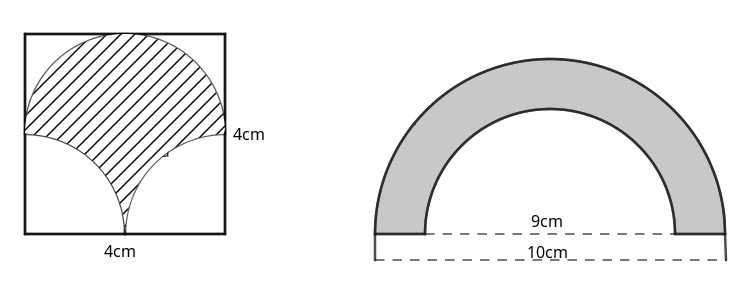
\includegraphics[scale=0.5]{mianji}
\end{center}

\question[6] 解方程.

 $1.5x+20\% x=5.95$ \hspace{3cm} $0.8x-20\% =3$ \hspace{3cm} $\dfrac{1}{2}:\dfrac{1}{8}=\dfrac{3}{2}:x$

\begin{minipage}{0.3\textwidth}
	解:\cyan
	1.5x+20\% x =5.95\\
	1.5x+0.2x =5.95\\
	1.7x =5.95\\
	x =3.5	
\end{minipage}
\begin{minipage}{0.4\textwidth}
	解:\cyan
	0.8x-20\% =3\\
	0.8x=3.2\\
	x =4	
\end{minipage}
\begin{minipage}{0.3\textwidth}
	解:\cyan
	$\dfrac{1}{2}:\dfrac{1}{8}=\dfrac{3}{2}:x\\
	\dfrac{1}{2}x=\dfrac{3}{16}\\
	x =\dfrac{3}{8}$
\end{minipage}

\question[8] 递等式计算(能简算的要简算)

$38\times \dfrac{1}{4}+17\times 0.25+45\times 25\%$ \hspace{4cm} $5\dfrac{4}{5}+\dfrac{7}{8}-1\dfrac{4}{5}+0.125$\\
$\dfrac{7}{12}\div [(\dfrac{7}{16}+\dfrac{1}{4})\times \dfrac{8}{33}]$ \hspace{5.4cm} $\dfrac{5}{8}\times 8.3-0.3\times 62.5\%$


\jiandac
\question[4] 一间房屋用边长5分米的正方形方砖铺地,要240块,如果改用每块是16平方分米的正方形方砖来铺,需要多少块?(用比例解)

\begin{solution}{\cyan
设需要$x$块,则
\[16x=5\times 5\times 240 \]
\[16x=25\times 240\]
\[x=375\]

答:需要375块.}
\end{solution}

\question[5] 老师用泥巴做了一个长方体,如果把这个长方体的长增加2cm,体积就增加40立方厘米;如果宽增加3cm,体积就增加90立方厘米;如果高增加4cm,体积就增加96立方厘米.求原来长方体的表面积是多少?

\begin{solution}{\cyan
	由题意可知,宽$\times$ 高=40$\div$ 2=20(平方厘米)\\
	长$\times$ 高=90$\div$ 3=30(平方厘米)\\
	长$\times$ 宽=96$\div$ 4=24(平方厘米)\\
	所以,2$\times$(长$\times$ 宽+长$\times$ 高+宽$\times$ 高)
	=2$\times$(20+30+24)=148(平方厘米)\\
	答:原来长方体的表面积是148平方厘米.}
\end{solution}


\jiandad
\question[5] 修一条公路,将总任务按5:6的比例分配给甲、乙两个工程队,甲队先修了630米,完成了分配任务的70\%,后来甲队调走,余下的任务由乙队修完,乙队一共修了多少米?

\begin{solution}{\cyan
\[630\div 70\%=630\div 0.7=900~\text{(米)}\]
\[900\div 5\times 6+(900-630)=1080+270=1350\text{(米)}\]

答:乙队一共修了1350米.}
\end{solution}


\question[5] 有A、B两个水桶,都装有水,A桶底面半径3分米,水面高4分米;B桶底面半径2分米,水面高3分米.现在往两个水桶内倒入等量的水,使得两个水桶的水面一样高,两个水桶内各应倒入水多少立方分米?

\begin{solution}{\cyan
设两个水桶水面高度为$x$分米,则由题意
\[3.14\times 3^{2}\times (x-4)=3.14\times 2^{2}\times (x-3),\text{解得}x=4.8\]
A桶内应倒入:$3.14\times 3^{2}\times 4.8=135.648$(立方分米)\\
B桶内应倒入:$3.14\times 2^{2}\times 4.8=60.288$(立方分米)	}
\end{solution}


\jiandae
\question[5] 五位裁判员给一名体操运动员评分后,去掉一个最高分和一个最低分,平均得9.58分;只去掉一个最高分,平均得9.46分;只去掉一个最低分,平均得9.66分.这个运动员的最高分与最低分相差多少?

\begin{solution}{\cyan
	\[9.46\times 4-9.58\times 3=9.1\]
	\[9.66\times 4-9.58\times 3=9.9\]
	\[9.9-9.1=0.8(\text{分})\]
	答:这个运动员的最高分与最低分相差0.8分.}
\end{solution}


\question[5] 市场鸡蛋按个数计价,一商贩以每个0.24元购进一批鸡蛋,但在贩运过程中,不慎碰坏了16个,剩下的蛋以每个0.28元售出,结果获利11.2元,问商贩当初买进多少个鸡蛋?

\begin{solution}{\cyan
		设商贩收购的鸡蛋共有$x$个,则购买时的总费用为$0.24x$元,销售的总价为$0.28(x-16)$元,由题意得:
		\[0.28(x-16)-0.24x=11.2\]解得$x=392$\\
		答:商贩当初买进392个鸡蛋.}
\end{solution}

\jiandaf
\question 某商场在春节期间开展优惠活动:\\
(1)如果一次购物不超过200元,不予折扣;\\
(2)如果一次购物超过200元,但不超过500元(含500元)的,按标价给予九折优惠,也就是按定价的90\%出售;\\
(3)如果一次购物超过500元,其中500元按第(2)条给予优惠,超过500元的部分给予八折优惠.\\
王老师两次去商场购物,分别付款160元和360元.\\
(1)王老师第二次购物商品的标价是多少元?\\
(2)如果王老师一次性购买这两次买到的商品,可以比已经用去的钱节省多少元?

\begin{solution}{\cyan
	(1)$360 \div 90\%=400(\text{元})$

	答:王老师第二次购物商品的标价是400元.
	
	(2)$160+400=560(\text{元})\\500 \times 90\%+(560-500)\times 80\%=498(\text{元})\\
	(160+360)-498=22(\text{元})$\\
	答:可以比已经用去的钱节省22元.}
\end{solution}

\end{questions}

\end{document}
